\documentclass[9pt,twocolumn,twoside,]{pnas-new}

% Use the lineno option to display guide line numbers if required.
% Note that the use of elements such as single-column equations
% may affect the guide line number alignment.


\usepackage[T1]{fontenc}
\usepackage[utf8]{inputenc}
% Pandoc syntax highlighting
\usepackage{color}
\usepackage{fancyvrb}
\newcommand{\VerbBar}{|}
\newcommand{\VERB}{\Verb[commandchars=\\\{\}]}
\DefineVerbatimEnvironment{Highlighting}{Verbatim}{commandchars=\\\{\}}
% Add ',fontsize=\small' for more characters per line
\usepackage{framed}
\definecolor{shadecolor}{RGB}{248,248,248}
\newenvironment{Shaded}{\begin{snugshade}}{\end{snugshade}}
\newcommand{\AlertTok}[1]{\textcolor[rgb]{0.94,0.16,0.16}{#1}}
\newcommand{\AnnotationTok}[1]{\textcolor[rgb]{0.56,0.35,0.01}{\textbf{\textit{#1}}}}
\newcommand{\AttributeTok}[1]{\textcolor[rgb]{0.13,0.29,0.53}{#1}}
\newcommand{\BaseNTok}[1]{\textcolor[rgb]{0.00,0.00,0.81}{#1}}
\newcommand{\BuiltInTok}[1]{#1}
\newcommand{\CharTok}[1]{\textcolor[rgb]{0.31,0.60,0.02}{#1}}
\newcommand{\CommentTok}[1]{\textcolor[rgb]{0.56,0.35,0.01}{\textit{#1}}}
\newcommand{\CommentVarTok}[1]{\textcolor[rgb]{0.56,0.35,0.01}{\textbf{\textit{#1}}}}
\newcommand{\ConstantTok}[1]{\textcolor[rgb]{0.56,0.35,0.01}{#1}}
\newcommand{\ControlFlowTok}[1]{\textcolor[rgb]{0.13,0.29,0.53}{\textbf{#1}}}
\newcommand{\DataTypeTok}[1]{\textcolor[rgb]{0.13,0.29,0.53}{#1}}
\newcommand{\DecValTok}[1]{\textcolor[rgb]{0.00,0.00,0.81}{#1}}
\newcommand{\DocumentationTok}[1]{\textcolor[rgb]{0.56,0.35,0.01}{\textbf{\textit{#1}}}}
\newcommand{\ErrorTok}[1]{\textcolor[rgb]{0.64,0.00,0.00}{\textbf{#1}}}
\newcommand{\ExtensionTok}[1]{#1}
\newcommand{\FloatTok}[1]{\textcolor[rgb]{0.00,0.00,0.81}{#1}}
\newcommand{\FunctionTok}[1]{\textcolor[rgb]{0.13,0.29,0.53}{\textbf{#1}}}
\newcommand{\ImportTok}[1]{#1}
\newcommand{\InformationTok}[1]{\textcolor[rgb]{0.56,0.35,0.01}{\textbf{\textit{#1}}}}
\newcommand{\KeywordTok}[1]{\textcolor[rgb]{0.13,0.29,0.53}{\textbf{#1}}}
\newcommand{\NormalTok}[1]{#1}
\newcommand{\OperatorTok}[1]{\textcolor[rgb]{0.81,0.36,0.00}{\textbf{#1}}}
\newcommand{\OtherTok}[1]{\textcolor[rgb]{0.56,0.35,0.01}{#1}}
\newcommand{\PreprocessorTok}[1]{\textcolor[rgb]{0.56,0.35,0.01}{\textit{#1}}}
\newcommand{\RegionMarkerTok}[1]{#1}
\newcommand{\SpecialCharTok}[1]{\textcolor[rgb]{0.81,0.36,0.00}{\textbf{#1}}}
\newcommand{\SpecialStringTok}[1]{\textcolor[rgb]{0.31,0.60,0.02}{#1}}
\newcommand{\StringTok}[1]{\textcolor[rgb]{0.31,0.60,0.02}{#1}}
\newcommand{\VariableTok}[1]{\textcolor[rgb]{0.00,0.00,0.00}{#1}}
\newcommand{\VerbatimStringTok}[1]{\textcolor[rgb]{0.31,0.60,0.02}{#1}}
\newcommand{\WarningTok}[1]{\textcolor[rgb]{0.56,0.35,0.01}{\textbf{\textit{#1}}}}

% tightlist command for lists without linebreak
\providecommand{\tightlist}{%
  \setlength{\itemsep}{0pt}\setlength{\parskip}{0pt}}


% Pandoc citation processing
%From Pandoc 3.1.8
% definitions for citeproc citations
\NewDocumentCommand\citeproctext{}{}
\NewDocumentCommand\citeproc{mm}{%
  \begingroup\def\citeproctext{#2}\cite{#1}\endgroup}
\makeatletter
 % allow citations to break across lines
 \let\@cite@ofmt\@firstofone
 % avoid brackets around text for \cite:
 \def\@biblabel#1{}
 \def\@cite#1#2{{#1\if@tempswa , #2\fi}}
\makeatother
\newlength{\cslhangindent}
\setlength{\cslhangindent}{1.5em}
\newlength{\csllabelwidth}
\setlength{\csllabelwidth}{3em}
\newenvironment{CSLReferences}[2] % #1 hanging-indent, #2 entry-spacing
 {\begin{list}{}{%
  \setlength{\itemindent}{0pt}
  \setlength{\leftmargin}{0pt}
  \setlength{\parsep}{0pt}
  % turn on hanging indent if param 1 is 1
  \ifodd #1
   \setlength{\leftmargin}{\cslhangindent}
   \setlength{\itemindent}{-1\cslhangindent}
  \fi
  % set entry spacing
  \setlength{\itemsep}{#2\baselineskip}}}
 {\end{list}}
\usepackage{calc}
\newcommand{\CSLBlock}[1]{#1\hfill\break}
\newcommand{\CSLLeftMargin}[1]{\parbox[t]{\csllabelwidth}{#1}}
\newcommand{\CSLRightInline}[1]{\parbox[t]{\linewidth - \csllabelwidth}{#1}\break}
\newcommand{\CSLIndent}[1]{\hspace{\cslhangindent}#1}


\templatetype{pnasresearcharticle}  % Choose template

\title{Variations spatio-temporelles de la biodiversité des lépidoptères
au Québec}

\author[a]{Marika Roberge}
\author[a]{Bertrand Labrecque}
\author[a]{Juliette Boulet-Thomas}

  \affil[a]{Faculté des sciences, Département de biologie, 2500
Boulevard de l'Université, Sherbrooke, Québec, J1K 2R1}


% Please give the surname of the lead author for the running footer
\leadauthor{}

% Please add here a significance statement to explain the relevance of your work
\significancestatement{}


\authorcontributions{}



\correspondingauthor{\textsuperscript{} }

% Keywords are not mandatory, but authors are strongly encouraged to provide them. If provided, please include two to five keywords, separated by the pipe symbol, e.g:
 \keywords{  lepidopteres |  communautés |  variation
temporelle |  variation spatiale  } 

\begin{abstract}
Ce rapport explore l'évolution de la diversité des lépidoptères au
Québec à partir d'environ 150 ans de données de présence. Trois analyses
ont été menées : (1) la variation temporelle de la richesse spécifique,
(3) les changements de répartition de Papilio canadensis, et (3)
l'évolution spatio-temporelle de la diversité. Les résultats révèlent
une hausse marquée des observations au fil du temps, probablement liée à
l'essor de la science participative. Des cartes spatio-temporelles
montrent une couverture accrue et une diversité croissante dans le sud
du Québec. Ces tendances soulignent l'importance de considérer les biais
d'échantillonnage pour mieux distinguer les effets réels des
perturbations environnementales.
\end{abstract}

\dates{This manuscript was compiled on \today}
\doi{\url{www.pnas.org/cgi/doi/10.1073/pnas.XXXXXXXXXX}}

\begin{document}

% Optional adjustment to line up main text (after abstract) of first page with line numbers, when using both lineno and twocolumn options.
% You should only change this length when you've finalised the article contents.
\verticaladjustment{-2pt}



\maketitle
\thispagestyle{firststyle}
\ifthenelse{\boolean{shortarticle}}{\ifthenelse{\boolean{singlecolumn}}{\abscontentformatted}{\abscontent}}{}

% If your first paragraph (i.e. with the \dropcap) contains a list environment (quote, quotation, theorem, definition, enumerate, itemize...), the line after the list may have some extra indentation. If this is the case, add \parshape=0 to the end of the list environment.

\acknow{}

\section{Introduction et questions de
recherche}\label{introduction-et-questions-de-recherche}

Les lépidoptères, en tant qu'indicateurs sensibles à la température et
aux changements environnementaux (1, 2), sont particulièrement utiles
pour évaluer les effets des perturbations anthropiques, notamment les
changements climatiques et l'altération des habitats. Au Québec,
plusieurs espèces pourraient voir leur aire de répartition modifiée,
soit par l'expansion d'espèces thermophiles vers le nord, soit par un
recul des espèces froid-adaptées.\\
Dans ce contexte, nous avons étudié l'évolution de la diversité des
lépidoptères au Québec, à la fois dans le temps et dans l'espace, en
nous basant sur les données de présence collectées depuis environ 150
ans. L'objectif principal est d'évaluer les changements dans la
diversité des lépidoptères au Québec à travers ces deux dimensions.
Ainsi, la première analyse se pose la question suivante : comment la
richesse spécifique des lépidoptères a-t-elle évolué au fil des années ?
La deuxième analyse cherche à répondre à la question suivante : comment
la répartition de Papilio canadensis a-t-elle changé au cours du temps
et dans l'espace au Québec ? Enfin, la troisième analyse s'interroge sur
: comment la diversité et la répartition des lépidoptères ont-elles
évolué au fil du temps et selon les régions du Québec ?\\
Ces résultats permettront de discuter des mécanismes potentiels à
l'origine des patrons observés, entre biais d'échantillonnage et signaux
biologiques réels, et d'évaluer si la composition des communautés de
lépidoptères au Québec reflète une transformation de la biodiversité
entomologique.

\section{Méthode et résultats
d'analyse}\label{muxe9thode-et-ruxe9sultats-danalyse}

Pour la première analyse, le graphique présenté ici (Fig. 1) illustre
l'évolution du nombre d'espèces uniques de lépidoptères observées au fil
des différentes années au Québec. Ce graphique permet de visualiser les
tendances et fluctuations dans la diversité des espèces le long de la
ligne du temps dans la province. Cette analyse repose sur un total de XX
XXX observations valides réparties entre 1859 et 2024.

Le choix d'illustrer le nombre d'espèces uniques de lépidoptères permet
de mieux refléter la diversité réelle des espèces observées, en excluant
les doublons et les variations dues à la fréquence des observations. Par
exemple, si une même espèce est observée plusieurs fois dans une année,
elle ne sera comptée qu'une seule fois, offrant ainsi une vision plus
précise des tendances de diversité. Cela permet également d'analyser les
fluctuations des populations et l'impact des facteurs environnementaux,
comme une variation climatique, sur la présence de certaines espèces.

\begin{Shaded}
\begin{Highlighting}[]
\FunctionTok{library}\NormalTok{(targets)}
\FunctionTok{tar\_load}\NormalTok{(graphique\_diversite)}
\end{Highlighting}
\end{Shaded}

\begin{figure}
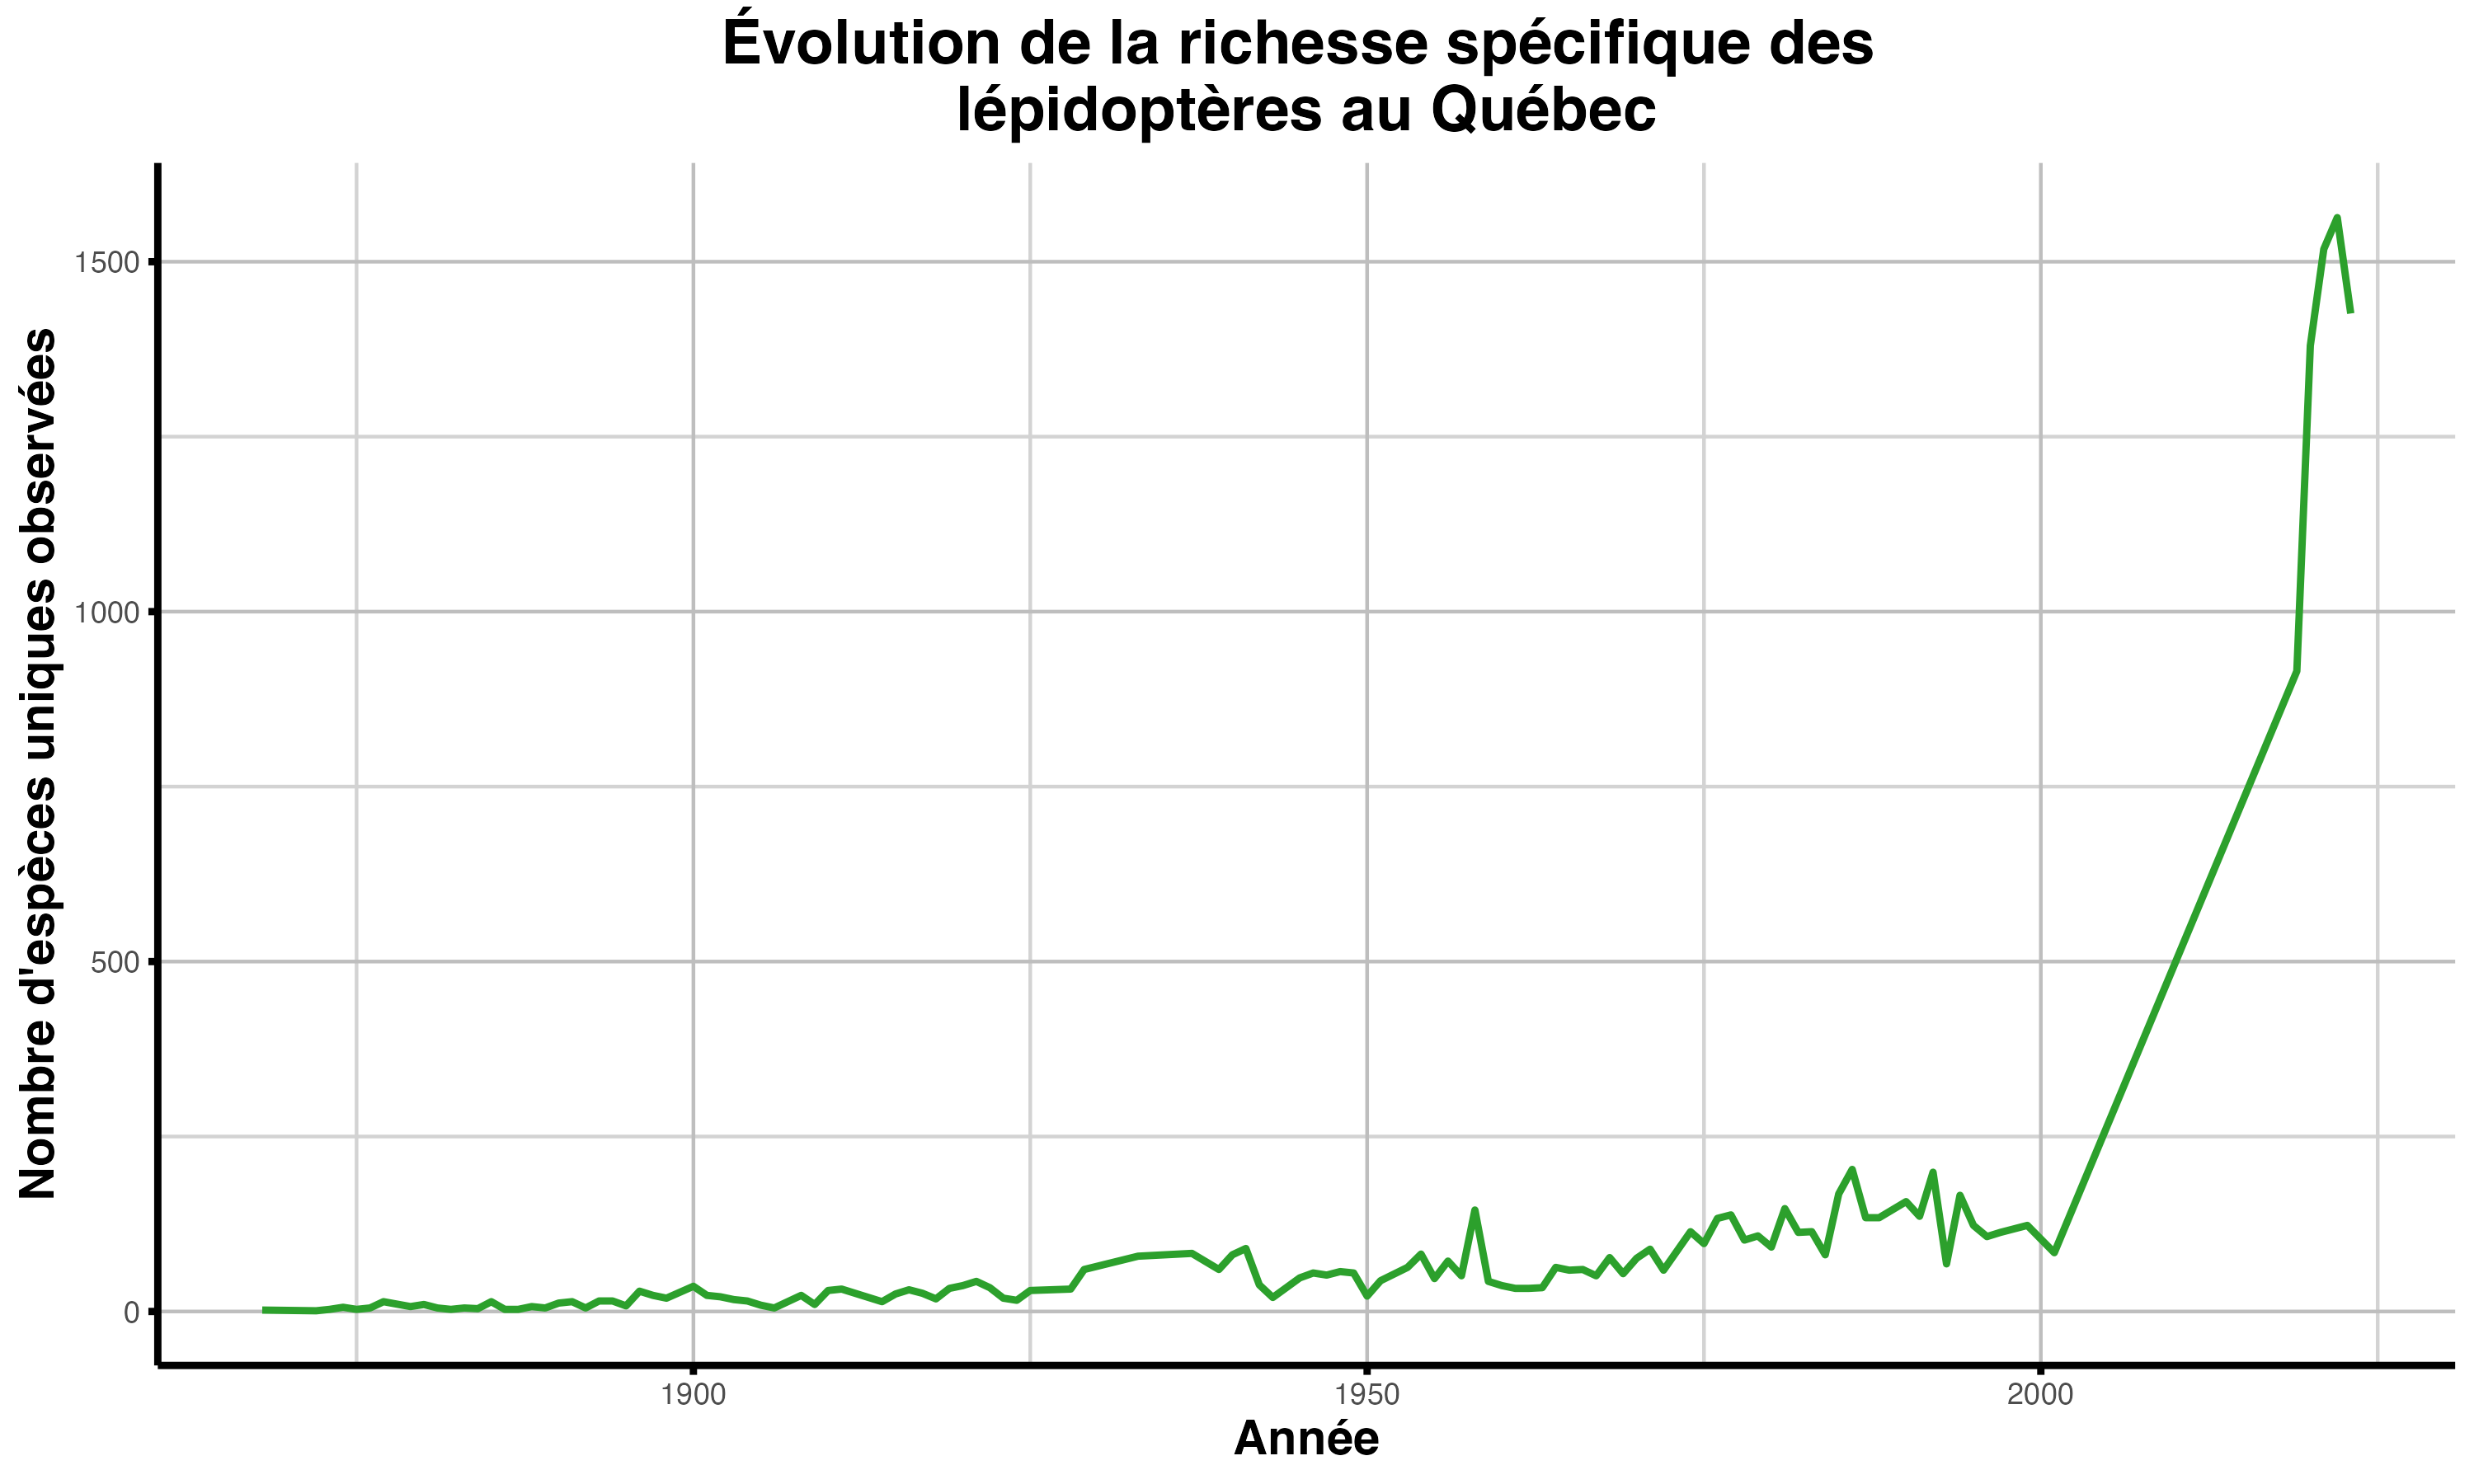
\includegraphics[width=0.9\linewidth]{Rapport/graphique_biodiversite} \caption{Variation du nombre d'espèces de lépidoptères au Québec en fonction du temps.}\label{fig:fig_graphique_biodiversite}
\end{figure}

On y observe une augmentation relativement lente et stable du nombre
d'espèces identifiées jusqu'au début des années 2000, suivie d'une
hausse extrêmement marquée à partir de 2005-2010, atteignant plus de
1500 espèces uniques observées.

Comme deuxième analyse, elle porte sur une espèce commune au Québec,
\emph{Papilio canadensis}, communément appelé Papillon tigré du Canada
(Fig. 2).

\begin{figure}

{\centering 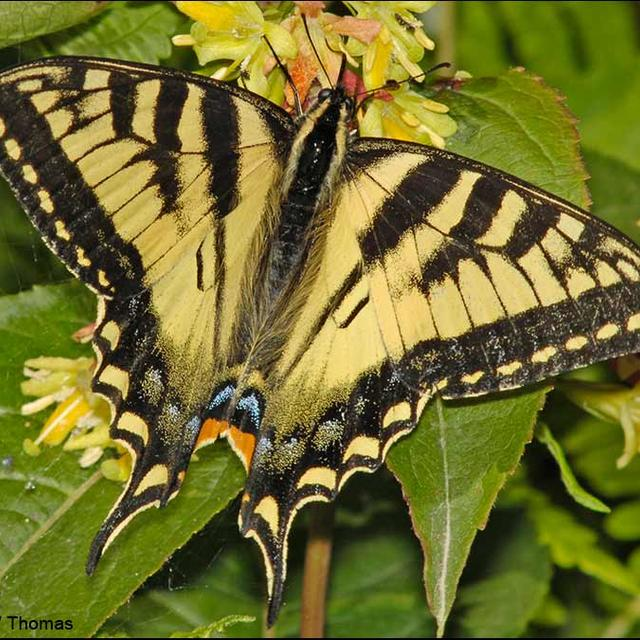
\includegraphics[width=0.8\linewidth]{Rapport/Papilio_canadensis} 

}

\caption{Papillon tigré du Canada (*Papilio canadensis*) observé dans son habitat naturel.}\label{fig:fig-papilio}
\end{figure}

Cette espèce est présente dans toutes les provinces et territoires du
Canada. Pour le Québec, on peut la trouver de la frontière à 100 km à
l'ouest de Radisson. Ce papillon est parfait pour l'étude, car il couvre
une grande partie du Québec et est facilement reconnaissable, ce qui en
fait un spécimen parfait pour une étude sur la biodiversité des
lépidoptères dans le temps au Québec (3).

L'analyse portant sur l'espèce permet de décrire comment la répartition
de \emph{Papilio canadensis} change dans le temps et l'espace.

\begin{Shaded}
\begin{Highlighting}[]
\FunctionTok{tar\_load}\NormalTok{(graphique\_points)}
\end{Highlighting}
\end{Shaded}

Les données d'observation de \emph{Papilio Canadensis} ont été combinées
en 4 groupes pour obtenir une meilleure visualisation des observations
dans le temps (Fig. 3). Ces groupes sont de 1859 à 1900, de 1900 à 1950,
de 1950 à 2000 et de 2000 à 2023, soit la dernière année comportant les
données. Ces tranches de temps ont été choisies afin de limiter le
nombre de graphiques produits et d'avoir une meilleure compréhension de
l'évolution au fil des siècles. Un système de présence-absence a été
utilisé pour l'ensemble des 50684 sites d'observation. Une marque sur le
graphique indiquera si le papillon a été observé sur ce site dans
l'intervalle de temps définit.\\
Il y a beaucoup plus d'observations avec le temps, soit 7 entre 1859 et
1900, 86 entre 1901 et 1950, 617 entre 1951 et 2000 et 923 entre 2001 et
2023. Entre 1901 et 1950, il y a déjà des observations près de
Waskaganish, ces observation seront de plus en plus au nord après ces
années. Les observations les plus au nord seront dans les environs de
Radisson. On remarque une diminution des observations dans le centre du
Québec entre la carte 3 et la carte 4. Les observation de la carte 4
sont beaucoup plus concentrées dans la région du Saint-Laurent et dans
le sud-ouest alors que celles de la carte 3 sont plus concentrées a
centre de la province.

Maintenant, dans cette section, nous analysons l'évolution de la
biodiversité des lépidoptères au fil du temps à travers plusieurs
visualisations. Nous allons créer des cartes et des graphiques pour
observer les variations et tendances.\\
Pour l'étude de la biodiversité des lépidoptères dans le temps et
l'espace, une figure regroupant six cartes a été réalisée. Dans cette
figure, on observe la carte de la province du Québec qui est notre aire
d'étude principale. Les points géographiques de la base de données qui
sont à l'extérieur de la province ne sont pas pris en compte. La carte
la plus ancienne débute en 1875 et représente les données sur 25 ans,
soit de 1875 jusqu'à la fin de 1879, ces bonds de 25 ans de données vont
jusqu'aux données les plus récentes, soit en 2024. Cette image permet
donc de combiner une analyse temporelle (par tranche de 25 ans) et une
agrégation spatiale via une grille hexagonale. En effet, une grille
hexagonable est utilisée pour éviter les effets de bord qu'on a avec une
grille carrée. De plus, elle permet une meilleure agrégration spatiale.
La projection utilisée pour cette carte est EPSG 32198, qui est la
projection locale du Québec. Cela permet une représentation précise à
l'échelle régionale. Pour finir, une moyenne de nombre d'espèces par
cellule pour chaque période de temps a été fait. Ce qui donne une idée
plus stable et comparable de la diversité à travers le temps.\\
En conclusion, ces 6 cartes sont combinées en une seule image finale, ce
qui permet une comparaison visuelle claire de l'évolution
spatio-temporelle de la diversité spécifique au Québec. Ce qui est utile
visualiser les zones où la diversité augmente, diminue ou reste stable.

La Figure 4 ci-dessous montrent l'évolution de la biodiversité des
lépidoptères pour différentes périodes et critères.

\begin{Shaded}
\begin{Highlighting}[]
\FunctionTok{tar\_load}\NormalTok{(cartes\_diversite)}
\end{Highlighting}
\end{Shaded}

Ces cartes illustrent une augmentation progressive de la couverture
spatio-temporelle des données au fil des décennies. Plus on avance dans
le temps, plus le nombre de cellules remplies augmente, avec des données
qui deviennent à la fois plus denses, plus complètes et de plus grande
valeurs.

Un premier point à souligner est que la période allant de 1875 à 1899
comporte très peu de données, principalement concentrées autour des
grandes villes comme Montréal, Québec et Sherbrooke. La diversité
moyenne est entre faible à modérée, mais les données sont trop rares
pour en tirer des conclusions solides. Entre 1900-1934 et 1925-1949, on
remarque une progression lente de la couverture grâce à l'accumulation
graduelle de données d'échantillonnage. Par contre, l'effort demeure
limité, ce qui rend les valeurs de diversité peu fiables, à l'exception
des zones urbaines du sud qui sont mieux couvertes.

Entre 1950-1974 et 1975-1999, on remarque l'apparition de cellules de
couleur orangée. Le sud et l'ouest du Québec en dehors des zones
urbaines sont de plus mieux couvert. Il. y a une meilleure répartition
des données dans l'espace.

La majorité du sud du Québec est désormais bien couverte entre les
années 2000 et 2024, notamment autour des grands centres urbains et des
zones agricoles. On observe également une augmentation de la diversité,
illustrée par la présence accrue de cellules en oranger et jaune.

Enfin, pour la période la plus récente (2000-2024), la couverture
devient à la fois plus dense et plus étendue à l'échelle du territoire.
La diversité moyenne y est généralement plus élevée, ce qui reflète
probablement un important renforcement des efforts de suivi, en partie
grâce à l'émergence de bases de données participatives comme
iNaturalist.

\section{Discussion}\label{discussion}

Pour ce qui est de la première analyse, l'augmentation abrupte du nombre
d'espèces de lepidoptères depuis 2005 au niveau de la Figure 1 ne
reflète probablement pas une véritable explosion de la biodiversité des
lépidoptères, mais plutôt un effort d'échantillonnage et
d'identification beaucoup plus important au cours des deux dernières
décennies. En effet, plusieurs facteurs peuvent expliquer cette
tendance, notamment la montée en puissance de la science participative
(avec des plateformes comme iNaturalist et eButterfly), la
généralisation de l'utilisation des appareils photo numériques et des
outils numériques de reconnaissance d'espèces, ainsi qu'un intérêt
grandissant du public et des chercheurs pour la documentation de la
biodiversité (4). Ces observations concordent avec les résultats d'une
étude récente indiquant que l'augmentation des données disponibles sur
la biodiversité depuis le début des années 2000 s'explique en grande
partie par l'implication citoyenne croissante et par une couverture
spatiale et temporelle des relevés plus étendue (4).

Au niveau de la deuxième analyse, la figure 3 nous apprend les régions
où les papillons ont été observés à travers le temps. On peut constater
qu'il y a de plus en plus d'observations au travers des années, ce qui
est normal étant donné que le nombre d'observateurs a augmenté et les
outils de partage des données ont évolué. Il est intéressant de
constater qu'entre la carte 3 et la carte 4, on note une diminution de
la population au centre du Québec et une augmentation au sud du Québec
et proche de l'Ontario, et ce, malgré un nombre plus important
d'observateurs. Il pourrait s'agir d'une diminution de la population
dans cette région ou un moins grand effort d'échantillonnage. À part la
distribution géographique de l'espèce, cette carte manque d'information
pour avoir une meilleure compréhension de la situation. Par exemple, le
nombre d'observation par site et le nombre d'observateurs par tranche de
temps auraient pu être ajoutés, ce qui nous aurait aidés à faire un
meilleur portait de la population au fil du temps. Le nombre
d'observateurs nous aurait aussi aidés à connaître la relation entre
l'augmentation d'observation et l'effort d'observation.

Finalement, pour la troisième analyse, un des biais importants associés
à la carte de biodiversité spatio-temporelle réside dans l'augmentation
du nombre d'observations au fil du temps, ce qui est attendu étant donné
l'évolution des efforts d'échantillonnage. Toutefois, ces données
traduisent autant les dynamiques biologiques réelles que l'intensité
vriable de l'observation. En effet, les avancées technologiques récentes
(comme la génétique ou la modélisation climatique) permettent de mettre
en lumière des dynamiques écologiques auparavant invisibles, créant
ainsi un décalage interprétatif avec les méthodes historiques. Comme
souligné dans une étude, les bases de données naturalistes présentent un
effort d'échantillonnage inégal dans le temps et dans l'espace, ce qui
peut nuire à la représentativité écologique des cartes produites (5).

Cela soulève notamment des questions concernant l'interprétation des
zones identifiées comme peu diverisifiées (en rouge). Ces zones
reflètent-elles réellement une faible diversité biologique ou simplement
un manque d'effort d'échantillonnage? Ce questionnement est d'autant
plus pertinent lorsqu'on observe que le sud du Québec, mieux couvert par
les inventaires, présente aussi une diversité plus élevée (6). Par
ailleurs, à partir de 1975, on observe une stabilisation du nombre moyen
d'espèces dans plusieurs cellules, ce qui pourrait indiquer que l'effort
d'échantillonnage devient suffisant pour représenter de façon plus
fidèle la diversité locale.

\section{Conclusion}\label{conclusion}

Il demeure donc essentiel de tenir compte de l'effort d'échantillonnage
afin d'éviter de surévaluer les tendances à long terme en matière de
biodiversité.

\section{Références
bibliographiques}\label{ruxe9fuxe9rences-bibliographiques}

\showmatmethods
\pnasbreak

\phantomsection\label{refs}
\begin{CSLReferences}{0}{1}
\bibitem[\citeproctext]{ref-devictor_differences_2012}
\CSLLeftMargin{1. }%
\CSLRightInline{Devictor V, et al. (2012)
\href{https://doi.org/10.1038/NCLIMATE1347}{Differences in the climatic
debts of birds and butterflies at a continental scale}. \emph{Nature
Climate Change} 2:121--124.}

\bibitem[\citeproctext]{ref-parmesan_poleward_1999}
\CSLLeftMargin{2. }%
\CSLRightInline{Parmesan C, et al. (1999)
\href{https://doi.org/10.1038/21181}{Poleward shifts in geographical
ranges of butterfly species associated with regional warming}.
\emph{Nature} 399(6736):579--583.}

\bibitem[\citeproctext]{ref-layberry_butterflies_1998}
\CSLLeftMargin{3. }%
\CSLRightInline{Layberry RA, Hall PW, Lafontaine JD, Fowler JT (1998)
\emph{The {Butterflies} of {Canada}} (University of Toronto Press)
Available at: \url{https://www.jstor.org/stable/10.3138/j.ctt1287smw}
{[}Accessed April 22, 2025{]}.}

\bibitem[\citeproctext]{ref-mandeville_participatory_2023}
\CSLLeftMargin{4. }%
\CSLRightInline{Mandeville CP, Nilsen EB, Herfindal I, Finstad AG (2023)
\href{https://doi.org/10.1038/s43247-023-00906-2}{Participatory
monitoring drives biodiversity knowledge in global protected areas}.
\emph{Communications Earth \& Environment} 4(1):1--10.}

\bibitem[\citeproctext]{ref-navarro_modelisation_2021}
\CSLLeftMargin{5. }%
\CSLRightInline{Navarro C (2021) Modélisation spatio-temporelle de la
dynamique d'émergence de lépidoptères univoltins à partir de données
opportunistes.}

\bibitem[\citeproctext]{ref-hillebrand_generality_2004}
\CSLLeftMargin{6. }%
\CSLRightInline{Hillebrand H (2004)
\href{https://doi.org/10.1086/381004}{On the generality of the
latitudinal diversity gradient}. \emph{The American Naturalist}
163(2):192--211.}

\end{CSLReferences}



% Bibliography
% \bibliography{pnas-sample}

\end{document}
